
\documentclass[a4paper,10pt,fleqn]{article} % Definiert Papier = A4;
                                            % Schriftgrösse = 10Punkte;
                                            % Mathe.-Gl. Modus = linksbündig
                                            % (siehe http://lefti.amigager.de/latex/Aufbau.html)

\usepackage[utf8x]{inputenc}                % utf8x kann alle Textcodierungen interpretieren
\usepackage[T1]{fontenc} %Schriftcodierung mit UTF-8
\usepackage{textcomp} %Erweiterung von fontenc
\usepackage{lmodern} %Erweiterung des Zeichensatzes

\usepackage{graphics}                       % Package für Einfügen/Anpassen von Grafiken
\usepackage{graphicx}
\usepackage{wrapfig}                        % Package zum Einfügen von Textumflossenen Bilder

\usepackage[english,ngerman]{babel}         % ngerman = Neues Deutsch; babel = internationalisierung einschalten
\usepackage[babel,german=quotes]{csquotes}  % Deutsche Gänsefüssechen

\usepackage{hyperref}

\usepackage{amsmath}                        
\usepackage[all]{xy}
%\usepackage[xindy]{glossaries}
\usepackage{makeidx}
\usepackage{pdfpages}
\usepackage{graphicx}
\usepackage{printlen}

\usepackage{blindtext}
\usepackage{lipsum}

\usepackage{multicol}

\usepackage{multirow}

\usepackage{verbatim}

\usepackage{color}

\usepackage{eurosym}

%\usepackage{hyperref}
\usepackage{acronym}

\usepackage{enumitem}

\usepackage{setspace}

\usepackage{threeparttable} %benötigt um Fussnoten in einer Tabelle zu machen
\usepackage{longtable}


\usepackage{spreadtab} %benötigt um in Tabellen zu rechnen
\usepackage{numprint}

%Package damit eine Seite quer genommen werden kann
\usepackage{lscape}

%Damit man eine Zelle farbig markiert werden
\usepackage{colortbl}


%
% Rechnen in Tabellen. Zeichen für den Dezimalpunkt
%
\STsetdecimalsep{{.}}

\definecolor{darkgreen}{rgb}{0,0.6,0}
\usepackage{listings}
\lstset{language=[LaTeX]TeX}
\lstloadlanguages{TeX}
\lstset{basicstyle=\ttfamily\footnotesize,
        numbers=left,
        numberstyle=\tiny,
        numbersep=5pt,
        breaklines=true,
        texcsstyle=\color{black},
        backgroundcolor=\color{gray!10},
        %commentstyle=\color{darkgreen},
        %keywordstyle=\color{red}\bfseries,
        %stringstyle=\color{blue}\bfseries,
        frame=single,
        tabsize=2,
        rulecolor=\color{black!30},
        title=\lstname,
        escapeinside={\%*}{*)},
        breaklines=true,
        breakatwhitespace=true,
        framextopmargin=2pt,
        framexbottommargin=2pt,
        inputencoding=utf8x,
        extendedchars=true,
        literate={Ö}{{\"O}}1
                 {Ä}{{\"A}}1
                 {Ü}{{\"U}}1
                 {ü}{{\"u}}1
                 {ä}{{\"a}}1
                 {ö}{{\"o}}1 
       }
%
% hypersetup etwas genauer
%
\hypersetup{pdftex=true,
            hyperfigures=true,
            hyperindex=true,
            bookmarks=true,
            bookmarksopen=true,
            bookmarksnumbered=true,
            %pdfborder={0 0 0},
            hypertexnames=true,
            colorlinks=true,
            pagebackref=false,
            linktocpage=false,% link "`behing"'
            plainpages=false,
            linkcolor=black,%blue,
            %anchorcolor=black,% Color for anchor text.
            citecolor=black,%green,%Color for bibliographical citations in text.
            filecolor=black,%magenta,%Color for URLs which open local files.
            menucolor=black,%red,%Color for Acrobat menu items. pagecolor color red Color for links to other pages, but currently unused
            urlcolor=black,%red,
            pdfstartview=Fit,
            pdfview={XYZ null null null},
            pdfpagelabels,
            pageanchor=true,
            hypertexnames=false
           }
%
% hypersetup etwas rudimentärer
%
%{
    %colorlinks,
    %citecolor=black,
    %filecolor=black,
    %linkcolor=black,
    %urlcolor=black
%}

\usepackage{url}

\usepackage{cite}
\usepackage{apacite}

\usepackage{pdfpages}                        % Packet für PDF Dateimanipulation laden

\usepackage{fancyhdr}                        % http://en.wikibooks.org/wiki/LaTeX/Page_Layout#Customising_with_fancyhdr

\usepackage{siunitx}                         % benötigt um Tabellen nach einem . auszurichten


\bibliographystyle{apacite}


\pagestyle{fancy} %eigener Seitenstil
\fancyhf{} %alle Kopf- und Fusszeilenfelder bereinigen

\addtolength{\textwidth}{1.5cm}
\addtolength{\evensidemargin}{-5mm}
\addtolength{\oddsidemargin}{-5mm}

\addtolength{\headwidth}{1.5cm}

%\rhead{\setlength{\unitlength}{1mm}
%\begin{picture}(-2,7)
%    \includegraphics[width=35mm]{hslu_logo2.PNG}
%\end{picture}}

\fancyhead[L]{Projektarbeit: Autonomer Ballwerfer} %Kopfzeile links
\fancyhead[C]{} %zentrierte Kopfzeile
\fancyhead[R]{HSLU - T\&A}
%\fancyhead[R]{\includegraphics[scale=0.25]{hslu_logo2.PNG}}
\renewcommand{\headrulewidth}{0.4pt} % obere Trennlinie
\fancyfoot[L]{PREN Team 32}
\fancyfoot[C]{HS - 2014}
\fancyfoot[R]{\thepage}
\renewcommand{\footrulewidth}{0.4pt} % untere Trennlinie

%
% Anpassung der Darstellung des Literaturverzeichnis
%
\let\oldbibliography\thebibliography
\renewcommand{\thebibliography}[1]{%
  \oldbibliography{#1}%
  \setlength{\itemsep}{10pt}%
}
%
% Abbildungen und Tabellen nur mit Kurzform angeben
%
\addto\captionsngerman{
\renewcommand{\figurename}{Abb.}
\renewcommand{\tablename}{Tab.}
}
%
% Benötigt um von zwei Stellen im Text auf dieselbe Fusszeile zu referenzieren
%
\newcommand{\footnoteremember}[2]{%
  \footnote{#2\label{#1}}
  \newcounter{#1}
  \setcounter{#1}{\value{footnote}}
}
\newcommand{\footnoterecall}[1]{%
  \hyperref[#1]{\footnotemark[\value{#1}]}
} 
\makeatletter
\providecommand{\rowno}[1][__empty__]
{%
  \ifthenelse{\isundefined{\c@rowno}}
  {%
    \newcounter{rowno}
  }
  {}%
  	\ifthenelse{\equal{#1}{__empty__}}
 	 {%
       \stepcounter{rowno}%
     }
     {%
 	   \setcounter{rowno}{#1}%
     }%
  \therowno%
}
\makeatother
%
%\makeglossaries
%\include{wa/wa_glossar}
%
\newcommand{\myTitel}{Produktrecherche}
\begin{document}
    %
    % Deck- und Titelblatt
    %
    \begin{titlepage}
    \begin{center}     
        \parindent0pt{\Huge PREN 1}\\
        \vspace*{1.2cm}
        Yves Studer\\
        Thomas Wiss\\
        Livio Kunz\\
        Nikolaus Manser\\
        MatteoTrachsel\\
        Güdel Manuel\\
        Pascal Roth\\
        \vspace*{1.2cm}
        {\Huge \myTitel}\\
        \vspace*{1cm}
%        \begin{figure*}[h!]
%            \centering
%            \includegraphics[width=0.7\textwidth]{Sourcen/Bilder/WuerfelTitel}
%        \end{figure*}
        \vspace*{10cm}
        {\normalsize Hochschule Luzern - Technik \& Architektur}\\
        {\normalsize PREN 1}\\
        \vspace*{0.6cm}
        {\normalsize Horw, Hochschule Luzern - T\&A, \today}\\
    \end{center}
\end{titlepage}

    \begin{titlepage}
    \parindent0pt {\Huge PREN 1}\\
    \vspace*{0.7cm}
    \newline
    \begin{tabular}{ p{6cm} p{5cm}}
        Yves Studer                & Thomas Wiss \\
        Dorfstrasse 28             & Bachhüsliweg 4a \\
        6264 Pfaffnau              & 6042 Dietwil \\
        +41 79 705 48 88           & +41 79 604 93 61 \\
        yves.studer@stud.hslu.ch   & thomas.wiss@stud.hslu.ch \\
                                   & \\
        Livio Kunz                 & Niklaus Manser \\
        Hubelmatt 7                 & Brunnmattstrasse 11\\
        6206 Neuenkirch         & 6010 Kriens \\
        +41 79 811 53 03           & +41 77 405 58 56 \\
        livio.kunz@stud.hslu.ch    & niklaus.manser@stud.hslu.ch \\
                                   & \\
        Matteo Trachsel			   & Manuel Güdel \\
        Hofstrasse 4               & Riedtalstrasse 4\\
        6004 Luzern                & 4800 Zofingen\\
        +41 79 511 57 88           & +41 79 774 41 40 \\
        matteo.trachsel@stud.hslu.ch & manuel.guedel@stud.hslu.ch \\
        						   & \\
        Pascal Roth			       & \\
        Dorfstrasse 18			   & \\
        6275 Ballwil		       & \\
        +41 79 717 68 94	       & \\
        pascal.roth@stud.hslu.ch   & \\
    \end{tabular}
    \vspace*{1.7cm}
    \newline
    {\Huge Meilenstein 1 Dokumentation}\\
    \vspace*{1.2cm}\\
    {\normalsize Dozent: Markus Thalmann}\\
    \vspace*{0.2cm}\\
    {\normalsize Hochschule Luzern - Technik \& Architektur}\\
    {\normalsize Interdisziplinäre Projekarbeit 2014}\\
    \vspace*{2.3cm}
    \newline
    {\normalsize Horw, Hochschule Luzern - T\&A, \today}\\
\end{titlepage}

    %
    % Inhlatsverzeichnis umbenennen und anschliessend einen Seitenumbruch
    % 
    %\begin{tabular}{|p{1.2cm}|p{1.2cm}|p{6cm}|p{3cm}|} \hline
\textbf{Version} & \textbf{Datum} & \textbf{Änderung} & \textbf{Verantwortlicher}\\ \hline
v1.0 & 25.9.14 & Dokument erstellt & Yves Studer\\ \hline
 &  &   &  \\ \hline
 &  &   &  \\ \hline
\end{tabular}  
    \renewcommand{\contentsname}{Inhalt}
    \tableofcontents
    \newpage 
    
    \begin{landscape}
	\section{Recherche-Tabelle}	
		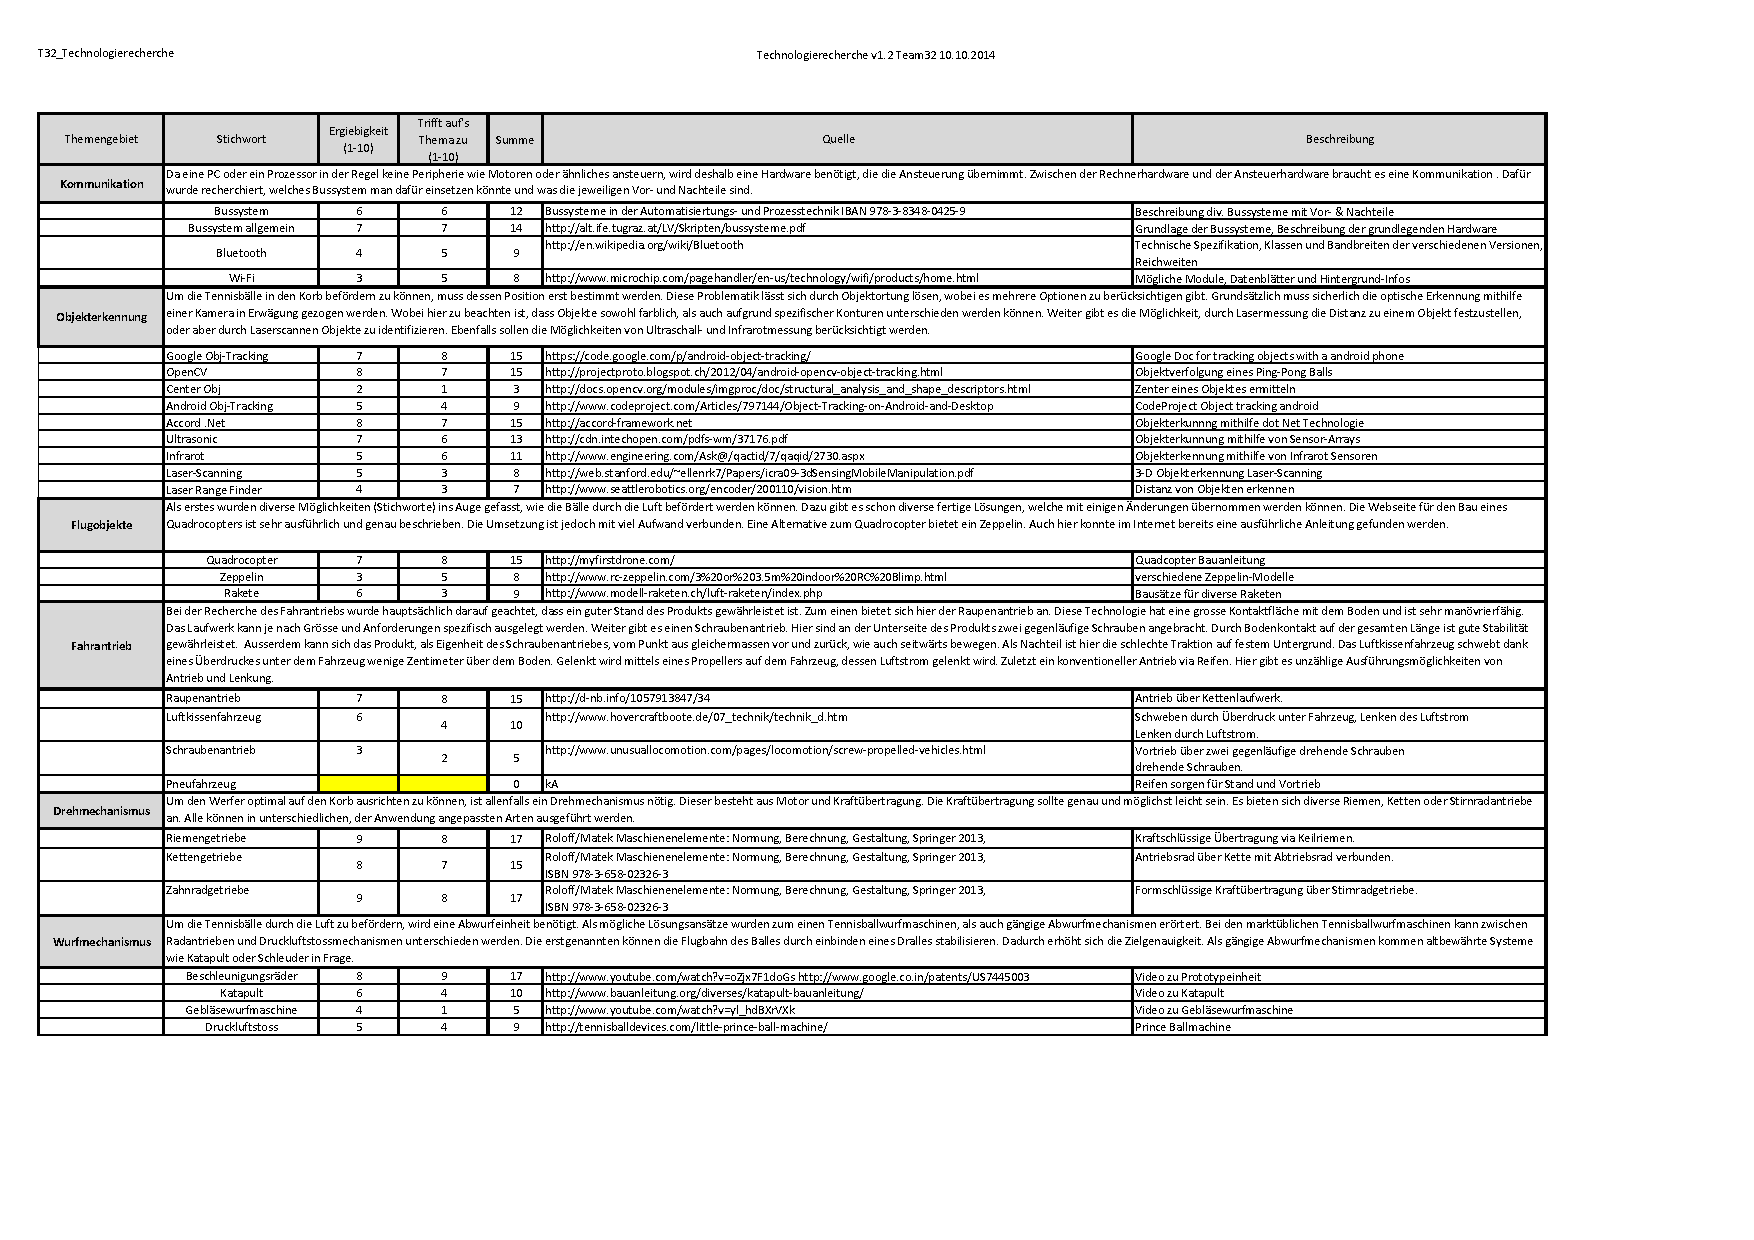
\includegraphics[page=1,scale=0.84,clip,trim=6.4mm 39mm 35mm 18mm]{Recherche/Extern/Produktrecherche.pdf}
		\newpage
		\includegraphics[page=2,scale=0.82,clip,trim=6.4mm 39mm 35mm 18mm]{Recherche/Extern/Produktrecherche.pdf}
\end{landscape} 
    \section{Drehmechanismus}
Falls der Werfer keine seitlichen Bewegungen ausführen kann, muss er sich mithilfe eines Drehmechanismus auf den Korb einstellen können. Diese Drehung kann auf verschiedene Weise realisiert werden. Die Anforderung ist, dass sich der Werfer bei Bedarf in einem bestimmten Winkelbereich nach links und rechts bewegen kann. Angetrieben von einem Elektromotor muss diese Verdrehung so präzise sein, dass ein exakter Wurf möglich ist. Weiter spielt nach den Produkteanforderungen auch die Geschwindigkeit der jeweiligen Verschiebung eine Rolle. Die gewählte Art der Kraftübertragung muss demnach geringe Trägheit aufweisen und kleine aber schnelle Bewegungen ermöglichen. 
 
\subsection{Riemengetriebe}
Bei Riemengetrieben wird die zu übertragende Kraft formschlüssig oder kraftschlüssig mit einem Zugmittel übertragen. Als kraftschlüssig übertragende Zugmittel werden Flach-, Keil- und Keilrippenriemen eingesetzt. Demgegenüber sind die Synchronriemen (Zahnriemen), die formschlüssig übertragen. \\
Ein grosser Vorteil dieser Technologie ist, dass sie in allen erdenklichen Lagen eingesetzt werden kann. Auch können mit nur einer Getriebestufe sehr grosse Übersetzungen erreicht werden. Der Aufbau ist im Vergleich einfach und preiswert. Als Nachteil zu werten ist die elastische Kraftübertragung. Bei hohen Anfahrmomenten Dehnt sich der Riemen um einen gewissen Wert, wobei Schlupf entstehen kann. Der Platzbedarf um eine gewisse Kraft zu übertragen ist grösser als bei anderen Prinzipien. Weiter zu beachten ist die elektrostatische Aufladung, die es durch Reibung gibt. 
 
\subsection{Kettengetriebe}
Kettengetriebe gehören ebenfalls zu den Zugmittelgetrieben. Überwiegend waagrecht verbaut sind sie eine Formschlüssigen Kraftübertragung zwischen Antriebs- und Abtriebswelle. \\
Gegenüber dem Riemengetriebe bieten sie den Vorteil der schlupffreien und konstanten Kraftübertragung. Bauartbedingt ist keine Vorspannung der Kette erforderlich. Dies führt zu geringeren Lagerbelastungen. Bei gleicher Belastbarkeit können sie kleiner ausgeführt werden. Ein Negativpunkt ist der Preis. Kettengetriebe sind teurer, als Riemengetriebe derselben Leistungsstufe.

\subsection{Zahnradgetriebe}
Diese Getriebe zeichnen sich durch kompakte Bauweise und hohen Wirkungsgrad aus. Auch hier herrscht ein Formschluss, also eine starre Verbindung ohne Schlupf. Zahnradgetriebe bestehen aus einem oder mehreren Zahnradpaaren. Je nach Art des Getriebes können Kraftumlenkungen in verschiedene Richtungen erreicht werden. Hier ist jedoch zu beachten, dass sich der Wirkungsgrad je nach Art wie die Kraftumlenkung erreicht wird, drastisch abnimmt. Mit nur einem Zahnradpaar können nicht so grosse Wellenabstände überbrückt werden, wie mit einem Zugmittelgetriebe. Durch mehrere Zahnradpaare, sind sehr grosse Drehzahl – Drehmoment Wandlungen möglich. Diese sind aber auch dementsprechend schwerer.  
    \subsection{Fahrantrieb}
Bei der Recherche des Fahrantriebs wurde hauptsächlich darauf geachtet, dass ein guter Stand des Produkts gewährleistet ist. Zum einen bietet sich hier der Raupenantrieb an. Diese Technologie hat eine grosse Kontaktfläche mit dem Boden und ist sehr manövrierfähig. Das Laufwerk kann je nach Grösse und Anforderungen spezifisch ausgelegt werden. Weiter gibt es einen Schraubenantrieb. Hier sind an der Unterseite des Produkts zwei gegenläufige Schrauben angebracht. Durch Bodenkontakt auf der gesamten Länge ist gute Stabilität gewährleistet.  Ausserdem kann sich das Produkt, als Eigenheit des Schraubenantriebes, vom Punkt aus gleichermassen vor und zurück, wie auch seitwärts bewegen. Als Nachteil ist hier die schlechte Traktion auf festem Untergrund. Das Luftkissenfahrzeug schwebt dank eines Überdruckes unter dem Fahrzeug wenige Zentimeter über dem Boden. Gelenkt wird mittels eines Propellers auf dem Fahrzeug, dessen Luftstrom gelenkt wird. Zuletzt ein konventioneller Antrieb via Reifen. Hier gibt es unzählige Ausführungsmöglichkeiten von Antrieb und Lenkung. 
    
    \subsection{Flugobjekte}
Als Flugobjekte wurden drei verschiedene Möglichkeiten ins Auge gefasst. Dazu zählt ein Quadcopter, eine Zeppelin und eine Rakete. Die Hauptschwierigkeit besteht bei der Steuerung der Objekte in der Flugphase. Eine weitere Teilschwierigkeit ist, eine berechenbare Flugbahn zu erreichen. 

\subsubsection{Quadrocopter}
\textbf{Vorteile}\\
Ein Quadrocopter kann als fertiger Baukasten gekaut und zusammengebaut werden. Die Flugsteuerung erfolgt über eine fertige Software.\\
\\
\textbf{Nachteile}\\
Die Steuerung des Quadrocopter ist sehr schwierig. Die Orientierung im Raum ist mit einer einfachen Software nicht möglich. Um eine bestimmte Flugbahn einzuhalten, brauchte man diverse Kameras, welche im Raum verteilt sind. Der ganze Quadrocopter und die Steuerung sind sehr kostenintensiv.\\
\\
\textbf{Umsetzbarkeit}\\
Eine Möglichkeit, für eine effiziente Umsetzung eines Quadrocopters in das Konzept ist fast 
Unmöglich. Die Kosten werden bei weitem überschritten. Die genaue Steuerung im Raum ist extrem schwierig. 

\subsubsection{Zeppelin}
\textbf{Vorteile}\\
Der Zeppelin kann als fertiger Baukasten gekauft werden. Die Modelle können der jeweiligen Hebelast angepasst werden. \\
\\
\textbf{Nachteile}\\
Der Auftriebskörper für eine kleine Masse zu heben, ist sehr gross. Die Steuerung des ganzen Zeppelins verläuft sehr träge.\\
\\
\textbf{Umsetzbarkeit}\\
Aus Platzgründen, welcher der Auftriebkörper benötigt, ist der Zeppelin sehr schwierig zu realisieren. \\
\\
\subsubsection{Rakete}
\textbf{Vorteile}\\
Sehr schneller Vortrieb des Wurfskörpers.\\
\\
\textbf{Nachteile}\\
Die Wurfbahn einer Rakete auf kleine Distanz ist fast unmöglich. \\
\\
\textbf{Umsetzbarkeit}\\
Die Umsetzung eines Raketenantriebes ist unmöglich.\\
\\
\\
Als erstes wurden diverse ins Auge gefasst, wie die Bälle durch die Luft befördert werden können. Dazu gibt es schon diverse fertige Lösungen, welche mit einigen Änderungen übernommen werden können. Die Webseite für den Bau eines Quadrocopters ist sehr ausführlich und genau beschrieben. Die Umsetzung ist jedoch mit viel Aufwand verbunden. Eine Alternative zum Quadrocopter bietet ein Zeppelin. Auch hier konnte im Internet bereits eine ausführliche Anleitung gefunden werden.
   
    \subsection{Object-Tracking – Objekt Verfolgung}
\subsubsection{Google Obj-Tracking}
Es wird mithilfe einer Android Smartphone, dessen Kamera und einem Adruino Uno Controller ein Objekt verfolgt. Dazu läuft auf dem Android Smartphone eine App die mithilfe der Kamera die Objekterkennung durchführt und die Informationen an den Controller weitergibt. Es ist eine Anleitung und Source Code vorhanden.

\subsubsection{OpenCV}
OpenCV ist eine OpenSource Bibliothek die eine Vielzahl von Bildverarbeitungsalgorithmen bereitstellt. Es wird beschrieben wie mithilfe von OpenCV und einer Android Kamera ein Objekt erkannt werden kann. Vorhanden sind Code Beispiele und Tutorials.

\subsubsection{Center an Object}
Code Beispiele wie man ein Objekt einmitten kann mithilfe von OpenCV. Code Beispiele sind in C++ und Python gegeben.

\subsubsection{Android Obj-Tracking}
Ein Tutorial für Object Tracking mit BoofCV. BoofCV ist eine Open-Source Bibliothek für Java. Hat Code Beispiele und Erklärungen wie man ein Objekt verfolgen kann.

\subsubsection{Accord.Net}
Accord.Net ist eine OpenSource Bibliothek für das .Net Framework. Es werden Code Beispiele angeboten und Tutorials
	
\subsubsection{Ultrasonic}
Beschreibt wie die Erkennung von Objekten mithilfe von Ultraschallsensoren.

\subsubsection{Infrarot}
Infrarot Sensoren geben einen Infrarot Lichtstrahl ab, ein Sensor erkennt dann die Rückstrahlung womit sich Objekte erkennen lassen. 

\subsubsection{Laser-Scanning}
Mithilfe eines Lasers können 3-D Modelle einer Umgebung erstellt werden indem viele Messungen durchgeführt werden und dann die einzelnen Punkte zu einem Gebilde zusammengesetzt werden.

\subsubsection{Laser-Range-Finder}
Laser Range Finder (LRF) können sehr gut dazu eingesetzt werden Distanzen zu bestimmen. Es werden die verschiedenen 

 
    \subsection{Versorgung}
Eine Möglichkeit um das Produkt mit Energie zu versorgen, ist ein Akkumulator. Es gibt verschiedene Typen: Blei-Akkus, Li-Ionen-Akku, Nickel-Cadmium-Akku (NiCd), Nickel-Metallhydird-Akku (NiMh). Jeder Typ hat verschiedene Vor- und Nachteile, die in der Tabelle \ref{tab:UebersichtVorNachTeil} ersichtlich sind.\\
\\
Ein grosser Vorteil besteht darin, dass ein Akkumulator nicht Teil des Produktegewichts ist. Wichtig für die anschliessende Auswahl des Akkumulators sind die Spannung, Strom, Kapazität des Akkumulators. In dieser Technologierecherche beschränkt man sich auf Eckdaten, die die Akkus auszeichnen, wie in der Tabelle \ref{tab:UebersichtAkku} ersichtlich.\\ 

\begin{table}[h!]
	\begin{tabular}{|p{1.5cm}|p{2.3cm}|p{3cm}|p{3cm}|} \hline
		          &\textbf{Energiedichte ($\frac{Wh}{kg}$})  & \textbf{Wirkungsgrad} & \textbf{Memory-Effekt}\\ \hline
		NiCd      & 40-60                                    & 70                    & Ja \\ \hline
		NiMH      & 70-90                                    & 70                    & Nein  \\ \hline
		Li-Ion    & 120-210                                  & 90                    & Nein \\ \hline
		Blei (Pb) & 30                                       & 60-70                 & Nein \\ \hline
	\end{tabular}
	\centering
	\caption{Übersicht der Akkumulatoren}
	\label{tab:UebersichtAkku} 
\end{table}

\begin{table}[h!]
	\begin{tabular}{|p{1.2cm}|p{5.3cm}|p{5.3cm}|} \hline
		          &\textbf{Vorteil}  & \textbf{Nachteil}\\ \hline
		NiCd      & \begin{itemize} \item Lange Lebensdauer \item Wartungsfreie Bauform \end{itemize} & \begin{itemize} \item In der EU verboten! \item Memory-Effekt (-> Kapazitätsverlust) \item Bei Defekt, sehr umweltschädlich \end{itemize} \\ \hline
		NiMH      & \begin{itemize} \item Hohe Kapazität \item Geeignet für Hochstromanwendungen \end{itemize} & \begin{itemize} \item Geringes Gewicht (kein Ballast) \item Hohe Selbstentladung 15\% pro Monat \end{itemize}   \\ \hline
		Li-Ion    & \begin{itemize} \item 5 Jahre funktionstüchtig \item Hohe Energiedichte \item Selbstentladung 1\% pro Monat \end{itemize} & \begin{itemize} \item Empfindlich auf falsche Behandlung \item Unter 1.5V kommt es zu Brandgefahr \item Geringes Gewicht (kein Ballast) \end{itemize} \\ \hline
		Blei (Pb) & \begin{itemize} \item 6 Jahre funktionstüchtig \item Hohe Strombelastbarkeit \item Hohes Gewicht (als Ballast) \end{itemize} & \begin{itemize} \item Selbstentladung 1\% pro Tag \item Nicht für mobilen Einsatz geeignet \end{itemize} \\ \hline
	\end{tabular}
	\centering
	\caption{Übersicht Vor- Nachteile der Akkumulatoren}
	\label{tab:UebersichtVorNachTeil} 
\end{table}

\subsubsection{Externe Versorgung}
In diesem Anschnitt ist die Versorgung mit Energie via Netzteil gemeint. Ein Vorteil eines Netzteils ist die stabile Energie- / Stromversorgung. Da eine Zuführung von einer Steckdose zum Spielfeld gewährleistet sein wird, fällt dies als Nachteil weg. Als Nachteil kann man jedoch auflisten, dass man das Netzteil nicht als Ballast verwenden kann. 

\subsubsection{Pneumatik}
Eine Versorgung mit Druckluft ist aufwendig und muss beim Spielfeld zur Verfügung gestellt werden. Ansonsten müsste man einen Kompressor mit Wartungseinheit organisieren. Zudem sind die Komponenten (Zylinder, Ventile, …) im Neuzustand seht teuer im Einkauf. 

\subsubsection{Hydraulik}
Die Versorgung mit Hydraulik-öl ist noch aufwendiger als jene mit Druckluft. Es muss ein eigenes System mit Pumpe, Schläuchen, Hydrauliköl und teuren Komponenten erstellt werden. Zudem entsteht bei einem Defekt resp. Unfall mit Hydrauliköl schnell ein grosser Sachschaden und erfordert einen grossen Reinigungsaufwand. 

      
    %
    % Start mit der eigentlichen Arbeit
    %    
\end{document}